
\subsection{Web applications}
\subsubsection{Design}
%-{\color{orange} “planning organizations should choose a participation platforms based on the capacities of their organization, the characteristics of the communities that are going to use the tool, user-community norms and rules, and the tool’s capabilities.”}\cite{Afzalan2017}\\
%-{\color{orange} “Discussing these factors with planners and decision makers, technologists, and communities who use the tools will add insights on identifying new considerations for implanting online participatory technologies”}\cite{Afzalan2017}\\
%-{\color{orange}“The geospatial Web 2.0, or Geoweb for short, is a collection of online location-enabled services and infrastructure that engages a wide range of stakeholders in mapping processes.” }\cite{Xing2015}\\
%-{\color{orange}Basic components: web participants, user groups, geoblog, blog components, blog profile, blog component profiel, blog description, time points and intervals, blog metrics. Relationships: generalization, composition, collaboration, possession.}\cite{Xing2015}\\
%-{\color{orange}“a general mashup architecture consists of three different participants that are logically and physically disjoint. THe generic architecture has the mashup client sitting on the top and the data sources and services sitting on the bottom. The middle tier is where the mashup logics reside. It should be noted that the mashup logics for generating mashed content could be either executed on the server or within the web browser.}\cite{Xing2015}\\
%-{\color{orange}Tagging: used GeoBLog with spatial extensions (server side scripting using JavaScript, Visual Studio 2010 2ithin the asp.net code).  Requires secure user authentication (login), access to post and transfer messages, and management tools programmes in asp.net.}\cite{Xing2015}\\
%-{\color{orange}Geoportal design: i. spatial database and data server; ii. geospatial web server; iii. Geospatial metadata catalogue server; iv. other catalogue server; v. download tool.\cite{Jiang2020}}\\
%-{\color{orange}“deconstructing the user-designer dichotomy… the boundary between user and designer is fluid and configured during the design process, and that users can have multiple identities. In addition to being users, they can perform activities traditionally ascribed to designers by dynamically participating in the ongoing design process.” “a user-centered design that deconstructs the traditional power relationship between designers and users through role hybridization by creating an environment where users or designers are able to shift from one role to another, effectively belonging to otherwise two distinc groups.” “designers can take the role of users, and users can participate in the design process, with constant interactions within and between the users and designers in order to combine and reconcile design ideas from the wto groups of users and designers.” “designer-user interaction models as a combination of interaction of designers, interaction of users and mutual interaction between designers and users with constant communication to increase knowledge sharing, crossing the social boundaries and deconstructing the design-user dichotomy to produce novel design artifacts and increase usefulness.”
%\cite{Karimzadeh2019}}\\
%-{\color{orange}“With inter-user communications capability built into the platform (in addition to the periodic face to face meetings and email exchanges), both users and designers were able to articulate their needs, comment on particular linguistic and geographic difficulties, deliberate together and suggest solutions from implementation.”\cite{Karimzadeh2019}}\\
%-{\color{orange}“In fact, code writers can be considered designers because they create software and algorithms that support evaluations and decisions directly impacting people’s lives. The filters that determine the selection and analysis of large and complex data sets on topics ranging from food access to health and nutrition originate from their coders’ specific world-views and reflect their implicit bias, inevitably shaping the outcome of research and surveys, which in turn influence policy decisions based on those enquiries.” \cite{Parasecoli2019}}\\
%-{\color{orange}“The dramatic rise of data visualization could be traced to hardware factors such as widespread use of high-resolution large desktop displays tied to powerful computers. Other important trends are the increased availability of vast data resources, familiarity with data management software, and innovative web-based software that support rapid display and update of visual information.”\cite{Shneiderman2020}}\\
%-{\color{orange}“The datavisualization process (also called ‘work flow’) starts with the identification of stakeholders and their insight needs. Just as a verbal math problem needs to be reformulated into a numerical math problem, the verbal or textual description of a real-world problem presented by a stakeholder must be operationalized (i.e., reformulated into a data visualization problem so that appropriate datasets, analysis and visualization workflows, and deployment options can be identified).”\cite{Borner2019}}\\
%-{\color{orange}“The task hierarchy provides insights about the ‘bigger-picture’ of each atomic task - a task that does not contain any subtasks - helping ensure that we always consider higher-level goals.”\cite{Zhang2019}}\\
%-{\color{orange}“As tasks often have dependency relationships with  each other, there can be a required task sequence. E.g., one has to view data before reasoning about it, and an overview visualization needs to be presented before selecting and examining outliers. Therefore, visualization tools should ont simply fulfill discrete tasks without providing for a natural flow between consecutive steps. Integrating task sequence information can help mingate the user’s mental burden and provide a better overall user experience.”\cite{Zhang2019}}\\
%-{\color{orange}“While many abstract tasks are similar (e.g. discover patterns and trends, reason about outliers), visualization tools often are used in a domain-specific context… We cannot simply peel off the domain-specific context, abstract to common data visualization tasks, and then design for those tasks. Context is key.”\cite{Zhang2019}}\\
%-{\color{orange}“When designing data visualization tools it is crucial to choose visual and interaction designs that solve the real-world problems of our target users. Task abstraction is widely used to support this process by characterizing user tasks as domain- and interface-agnostic abstract tasks for which design best practices are known.”\cite{Zhang2019}}\\
%-{\color{orange}THree step hierarchical task abstraction: “(1) understand the problems and data of domain users; (2) perform hierarchical task analysis to understand user tasks, goals, and the relationships among the tasks as part of a larger analysis process; and (3) abstract the user domain tasks.”\cite{Zhang2019}}\\
%-{\color{orange}“Once constructed, the hierarchical task and data type abstractions should inform visual encoding and interaction design.”\cite{Zhang2019}}\\
%
\subsubsection{Open Source}
%-{\color{orange}“To develop on an open source platform is extremely vital when huge databases are to be created and consulted regularly for region planning at different scales particularly satellite images and maps of their locations”.}\cite{Bhattacharya2018}\\
%-OGC Standards
%-{\color{orange}Trailblazers set the tone for future scalable impact and change. Foundational development and openness are key\cite{WEF2021}}\\
%-{\color{orange} “Transparency underpins integrity and legitimacy. Trailblazers have nothing to hide. They are working towards a better future and are transparent as to how their product road map will lead to better solutions over time.”\cite{WEF2021}}\\
%-{\color{orange}“Trailblazers share their technological knowledge and intellectual property with other players in the industry. THey recognize that it is more important to increase the pie than to increase only their share of it. From creative commons and open source tools to commercial arrangement, such as commercial licensing or training and support services, trailblazers find ways to push the market with their knowledge. They do this in a way that enables others to follow them towards a higher standard without compromising their competitive position.”\cite{WEF2021}}\\
%
\subsubsection{Data}
%\textbf{Volunteer generated information sources}\\
%-{\color{orange}VGI and geoweb: “there is mounting evidence that institutions can use VGI as a mechanism to build a local capacity to support collaboration, supplement traditional data sources, and inform decision making.” The VGI paradigm “Is enabled by teh GeoWeb, locatinoaware devices, and citizens acting as sensors, and their tools and resources for collecting and processing geographic information from volunteers are readily available.”}\cite{Xing2015}
%-{\color{orange}“VGI involves the creation and dissemination of geographic data provided voluntarily by individuals and overlaps with PPGIS in that both involve the investigation and identification of locations that are important to individuals.”\cite{Brown2012}}\\
%-{\color{orange}“PPGIS projects are often implemented to inform planning and policy issues while VGI systems may have no explicit purpose other than participant enjoyment.”\cite{Brown2012}}\\
%-{\color{orange}“Given well-defined insights needs, relevant datasets and other resources can be acquired. Data quality and coverage will strongly impact the quality of results, and much care must be taken to acquire the best dataset with data scales that support subsequent analysis and visualization.”\cite{Borner2019}}\\
%
%\textbf{Data harmoziation}
%-{\color{orange} Data harmonization: “Some geoportals not only provide data as they come from the original source, but they are also able to provide spatial data and geo-information coming from different sources into a common (i.e. standard) format… Data harmonization can help to receive, process, and exchange data, and to ensure interoperability, because the harmonized data and information are accessible to end users at their demands.” Federated approach: \cite{Jiang2020}}\\
%-{\color{orange}Federated approach: “participants to agree on common specifications in terms of metadata, data models, and service interfaces, typically based on international de-jure or de-facto standards.” Brokered approach “leveraged middleware between the client and the server tiers by addressing heterogeneity through mediation (i.e. of metadata and data models) and adaptation (i.e. of interfaces). In the brokered approach, the brokers as key component are dedicated to mediation and haronization. The brokered approach has been particularly appealing for those wanting to build Systems-of-systems, e.g. distributed infrastructures connecting systems, which keep their autonomy at a certain degree.” “Generally, the brokered approach is more effective in addressing variety and heterogeneity when central authority cannot be easily achieved.”\cite{Jiang2020}}\\
%-{\color{orange}Basic functionality: “metadata registry, data discovery through a catalogue service, data visualization, and data access.”{\color{red} See section 2.3.4 for more info}\cite{Jiang2020}}\\
%-{\color{orange}“A geospatial metadata catalogue provides data descriptions in terms of metadata (e.g. contributor, data type, language, contact point, keywords, and dataset identifier for data localization and indexing). In addition, the metadata catalogue is often used for implementing harmonized data discovery. Since users are typically interested in finding datasets matching specific constraints, the data discovery functionality is one of the basic functions that geoportals offer. SPecifically, geoportals providing data discovery generally allow searching datasets along the who, when, where and what axes, that is, by geo-location (where), data provider (who), time range (when), thematic layer, and keywords (what). The user interface provides graphical tools, like a bounding box on a map, to set spatial and temporal constraints. Moreover, users can be directed to a gazetteer, a thesaurus, or other knowledge bases for better scoping their query. Various approaches have been developed to enhance geoportal search capabilities, e.g. the use of thesauri, ontologies, and semantic text matching algorithms”.\cite{Jiang2020}}\\
%-{\color{orange}“Big data are posing challenges that are usually referred as V challenges: large Volume, high Velocity, and wide Variety. On the geoportal user interface side, they have an impact on discovering, visualizing, processing, and storing big Earth data. Specific challenges come from teh continuity of data updating, methods of data harmonization, and mulitple functionalities fro professional users.”\cite{Jiang2020}}\\
%-{\color{orange} Top down approach: “administrative approach”. Support “incorporate large amounts of spatial datasets and geo-information products, multi layered and multi types of data for earth sciences.” \cite{Jiang2020}}\\
%-{\color{orange}Top down approach: “administrative approach”. Support “incorporate large amounts of spatial datasets and geo-information products, multi layered and multi types of data for earth sciences.” \cite{Jiang2020}}\\
%-{\color{orange}Top down approach challenge: sustainability and homogeneity, insufficient searchability for nuanced use. Open Geographic Modeling System (OpenGMS) to combat this.\cite{Jiang2020}}\\
%-{\color{orange}“The data systems, where the geoportals connect, are leveraging different methods for coordination, in terms of federated coordination (top-down) and broker coordination (bottom.up). Both coordination solutions are able to connect distributed data servers and information systems, and to facilitate complex systems for solving big data storage, management, and assessment problems. The federated approach generally shows better performance, but it requires that participants agree on participating in the overall system bylaw or their own interests. If this is not available, a brokered approach is the only one that can be adopted. In addition, the brokered approach is better, if the requirements cannot be fully defined allowing one to select the best federal agreement. Therefore, a hybrid data system architecture for a complex data system is recommended for meeting the challenges posed by big data.”\cite{Jiang2020}}\\
%-{\color{orange}Data integration: “The discipline of data integration comprises the practices, architectural techniques and tools for achieving the consistent access and delivery of data across the spectrum of data subject areas and data structure types in the enterprise to meet the data consumption requirements of all applications and business processes.” (Gartner)\cite{Hintz2020}}\\
%-{\color{orange}“Performing temporal inference using disparate applications for each data source is challenging. Despite several advances in data interaction and visualization, device interoperability and data integration remains problematic.”\cite{Zhang2019}}\\
%
%
\textbf{Data access}\\
%-{\color{orange} Geoportal design: Spatial metadata catalogue server: ``The geospatial metadata catalogue provides metadata in accordance with OGC and ISO standards and is retreived by teh geoportal'' \cite{Jiang2020}}\\
%-{\color{orange} Geoportal design: other catalogue server ``Other catalogues could be supplemented by metadata catalogues for a data registry. A well-known catalogue is theGazetteer Service which can host a location-based feature dataset'' \cite{Jiang2020}}\\
%
\subsubsection{GIS design}
%-{\color{orange}“the design of the event model is composed of two parts: Spatiotemporal and Attribute information. Spatiotemporal information is polymerized by Feature, Temporal and Geometry. Among them, Temporal is composed of the time instant and time interval. Geometry is described by Position coordinate and Coordinate system, which belongs to Point, Line and Polygon. Attribute information is composed of Border type, Feature type, and Rss:Item; the model provides an extension of the elements by Rss:Item.”}\cite{Xing2015}\\
%-{\color{orange}Geoportal design: Spatial database and data server ``Spatial databases store and maintain the data that will be delivered. The database could be on the local server or distributed servers.''\cite{Jiang2020}}\\
%-{\color{orange}“data storage and management is one of the critical technical components for addressing the volume challenges of big data. Currently, relational databases (e.g. PostgreSQL), NoSQLs (e.g. MongoDB and HBase), and distributed file systems (e.g. Hadoop) are widely used for big data storage and management. These technologies are also important for geoportals, although the technical component for big data storage and management still requires more theoretical and practical developments.” \cite{Jiang2020}}\\
%
\subsubsection{Web services}
%-{\color{orange}Standards: Geoportals are usually compliant with several OGC standards, wtih some of the most popular ones being the Web Coverage Service (WCS), the Web Processing Service (WPS), the Web Coverage Processing Service (WCPS), the Web Map Service (WMS), the Web Feature Service (WFS), and the Catalog Service for Web (CSW). GeoServer\cite{Jiang2020}}\\
%-{\color{orange}Geoportal design: Geospatial web server: ``Geospatial web services provide greographic data to the user through forms of map data services uder the guidance of OGC and ISO standards. Open-source options for web services are capable of hosting these web services, e.g. GeoServer and MapServer \cite{Jiang2020}}\\
%Example:
%\begin{itemize}
%	\item Twitter map \cite{Fisher2014}
%	\item COVID visualization \cite{Shneiderman2020}: {Good design and professional practice is to show the sources of data, name the contributors to the visualization, and provide an email address for comments, corrections, and questions.\cite{Shneiderman2020}}{Example of Johns Hopkins University visualization of COVID data}.  {References of John Snow and WIlliam Playfairs addition to geodisplays to distill information and draw new spatial conclusions\cite{Shneiderman2020}}.{\color{orange}Use of spatial data to “persuade, understand current conditions, and predict future outcomes based on behaviors”.\cite{Shneiderman2020}} {Many references to additional display options (weather.com, microsoft power bi, esri, visual action, etc.}{\color{orange}“These widely used COVID-19 visualizations depend on maps, bar charts, line chars, and scrolling lists, however designing them to fit on small mobile-device displays requires skillful programming.”\cite{Shneiderman2020}}  
%\end{itemize}
%



%%%    DESIGN REFERENCE 
%\subsubsection{Graphic user interface}
%-{\color{orange}“The interactive graphical user interface (GUI) allows for data visualization manipulation and sharing.”}\cite{Bhattacharya2018}\\
%-{\color{orange}“The six areas should be covered on the geoportal interface are including metadata, data thumbnail, data description document, data sample, data entity (i.e. download link), and connections and groups. The goal of mode is to provide a more detailed description of the data on the geoportal and enable users enough information for faster data positioning and discovering.” Main elements of a geoportal.\cite{Jiang2020}}\\
%-{\color{orange}“A well-designed GUI is beneficial for interacting with the user and providing an easy-to-use experience and powerful visualized interactivities.”\cite{Jiang2020}}\\
%-{\color{orange}“Geoportals tend to prefer adopting an atlas-like user interface (using OpenLayers and Leaflet). THis may result in the requirement of visualizing geographic distributions of the data and of the functionality for visualized data selection. An atlas-like user interface, as the metaphor, is recommended for geoportal design.” Validation of openlayers and leaflet.\cite{Jiang2020}}\\
%-{\color{orange}“In order to address some Volume, Variety, and Velocity challenges on the user interface side, the next generation geoportals should specify the time-series investigation, graphs and charts for visual analytics, and 3D and 4D visualization widgets through dynamic visualization tools.”\cite{Jiang2020}}\\
%-{\color{orange}“For an effective presentation, the news must be shown in an informative, aesthetically pleasing manner, but this must not overwhelm the viewer.”\cite{Teitler2008}}\\
%-{\color{orange}“Because it is inevitable that multiple news stories will mention the same location, we also need a strategy for dealing with occlusion, since we do not want to place markers on top of each other.”\cite{Teitler2008}}\\
%-{\color{orange}Dynamic map labeling: “placing text labels tied to geographic coordinates on a map, usually requiring that some corner or edge of the label’s bounding box touch the coordinates associated with the label.”  Leverage a precomputed conflict graph (“labels correspond to nodes, and edges exist between labels that overlap”).\cite{Teitler2008}}\\
%-{\color{orange} “some occlusion of markers is tolerable, as long as the more significant story markers are placed above less significant markers. One exception to this rule is when markers exactly coincide - that is, when several stories mention the same geographic location. It is unacceptable to place markers at the exact same coordinates on the map, as users cannot infer that many stories refer to that location. This is often a problem with large cities, as they are a part of geographic focus of many news articles.” Spiral strategy: “this allows significant geographic locations to have more of their stories visible, at the expense of accuracy in marker placement. However, due to their regular shape, these spirals are usually easy to identify and do not contribute significantly to user confusion.”}{\color{purple} Ideally the inclusion of custom reference points/areas will alleviate this issue, though more popular POIs will likely include several concurrent news stories.}\cite{Teitler2008}\\
%-{\color{orange}“Many of the currently popular visualization follow the well-established Information Visualization Mantra: ‘Overview first, zoom and filter, then details-on-demand.’”\cite{Shneiderman2020}}\\
%-{\color{orange}Visual Information Seeking Mantra: overview first, zoom and filter, then details-on-demand\cite{Shneiderman1996}}\\
%-{\color{orange} Data types: 1D, 2D, 3D, temporal and multi-dimensional data, tree and network data). Includes detailed descriptions of these.\cite{Shneiderman1996}}\\
%-{\color{orange}Tasks: overview (“gain an overview of the entire collection”), zoom (“zoom in on items of interest”), filter (“filter out uninteresting items”), details-on-demand (“select an item or group and get details when needed”), relate (“view relationships among items”), history (“keep a history of actions to support undo, replay, and progressive refinement”), extract (“allow extraction of sub-collections and of the query parameters”).\cite{Shneiderman1996}}\\
%-{\color{orange}Multi-dimensional: “the interface representation can be 2-dimensional scattergrams with each additional dimension controlled by a slider.”	\cite{Shneiderman1996}}\\
%-{\color{orange} Multi-dimensional: “the interface representation can be 2-dimensional scattergrams with each additional dimension controlled by a slider.”\cite{Shneiderman1996}}\\
%-{\color{orange}Data Scales: “Data variables may have different scales (e.g., qualitative or quantitative), influencing which analyses and visual encoding can be used.”\cite{Borner2019}}\\
%-{\color{orange}Visualize “This step can be split into two mian activities: pick reference system (or base map) and design data overlay. The First activity is associated with selecting a visualization type, and the second activity is associated with mapping data records and variables to graphic symbols and graphic variables.”\cite{Borner2019}}\\
%-{\color{orange}Deploy “Different interface controls make diverse interactions possible: buttons, menus, and tabs support selection:; sliders and zoom controls let users filter by time, region, or topic: hover and double click help users retrieve details on demand; and multiple coordinated windows are connected via link and brush.”\cite{Borner2019}}\\
%-{\color{orange}Interpret: “Finally, the visualization is read and interpreted by its author(s) and/or stakeholder(s). This process includes the translating the visualization results into insights and stories that make a difference in the real-world application.”\cite{Borner2019}}\\
%
%\begin{figure}[H]
%	\centering
%	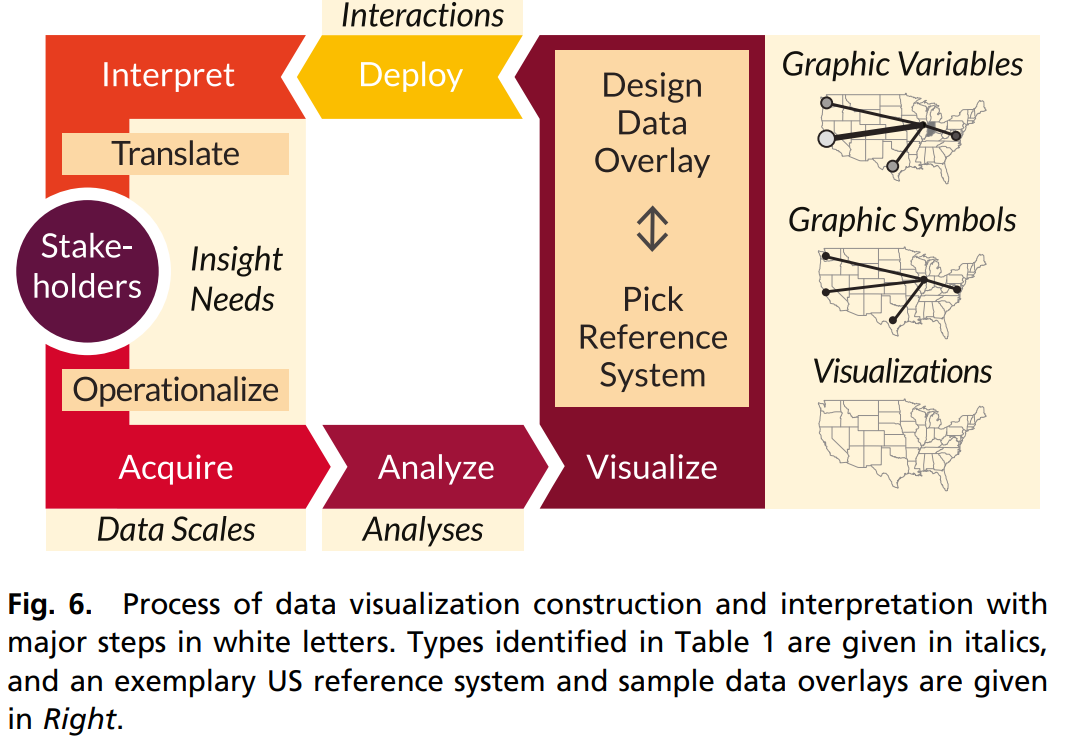
\includegraphics[width=.9\linewidth]{images/borner2019_figure6.png}
%	\caption{Process of data visualization construction and interpretation with major steps in white letters. Types identified in Table 1 are given in italics, and an exemplary US reference system and sample data overlays are given in Right. (Borner2019)}
%	\label{fig:borner2019_fig6}
%\end{figure}
%
%\subsubsection{Data manipuliation}
%-{\color{orange}Geoportals can also offer online processing functionalities, ranging from basic transformations (e.g. coordinate reference system re-projection, sub-setting, format mapping) to complex algorithms for classification, and statistical analysis. That may require an underlying infrastructure providing a workflow engine to orchestrate the multiple actions required to implement the required processing.”\cite{Jiang2020}}\\
%-{\color{orange}Spatial queries require indices (such as R-trees or quadtrees) for efficient execution.\cite{Lieberman2010}}\\
%-{\color{orange}Zoom: “smooth zooming helps users preserve their sense of position and context”.\cite{Shneiderman1996}}\\
%-{\color{orange}Filter: “By allowing users to control the contents of the display, users can quickly focus on their interests by eliminating unwanted items.''\cite{Shneiderman1996}}\\
%-{\color{orange}History: “It is rare that a single user action produces the desired outcome. Information exploration is inherently a process with many steps, so keeping the history of actions and allowing users to retrace their steps is important.”\cite{Shneiderman1996}}\\
%-{\color{orange}“Dynamic queries can reveal global properties as well as assist users in answering specific questions.”\cite{Shneiderman1996}}\\
%-{\color{orange}“dynamic visualizations: overview, zoom, filter, details on demand, relate (viewing relationships among items), history (keeping a log of actions to support undo, replay, and progressive refinement), and extract (access subcollections and query parameters)”\cite{Borner2019}}\\
%-{\color{orange}“Keim distinguishes zoom filter, and link and brush as well as projection and distortion techniques as a means to provide focus and context.”\cite{Borner2019}}\\
%-{\color{orange}“Brehmer and Munzner covers two main abstract visualization tasks. The first is ‘why’, which includes consume (present, discover, enjoy, produce, search (lookup, browse, locate, explore), and query (identify, compare, summarize). The second is ‘how,’ which consists of encode, manipulate (select, navigate, arrange, change, filter, aggregate), and introduce (annotate, import, derive, record).”\cite{Borner2019}}\\
%-{\color{orange}Other setup: “data and view specification (visualize, filter, sort, derive), view manipulation (select, manage, coordinate, organize), and process and provenance (record, annotate, share, guide).”\cite{Borner2019}}\\
%
%\subsubsection{Security}
%-{\color{orange}“some people might be concerned about sharing their identify in online environment or making their profile information visible, as they are worried about organizational and social threats”.}\cite{Afzalan2017}.\\
%-{\color{orange}“For implementing these common functionalities, additional functionalities are often required. For example, a geoportal should implement a subset of functionalities concerning privacy and security aspects, e.g. authentication, data access control, logging. Moreover, the geoportal administrators need dedicated management functionalities. \cite{Jiang2020}}\\
%
%
%\subsubsection{Products}
%-{\color{orange}Recommended services for geoportals: catalogue, preview, access, and online analysis and processing \cite{Jiang2020}}\\
%\textbf{RSS}\\
%-{\color{orange}“Publish/Subscribe has emerged as a communication paradigm able to facilitate the development of complex distributed applications in open network environments. THe strong decoupling it introduces between communication parties enables applications to publish information without being aware of the identities of potential receivers or even of their existence.  Similarly, it enables receivers to issue subscriptions that express their interests in messages with a given content regardless of the identity of their publishers.”}\cite{Xing2015}\\
%-{\color{orange} “GeoRSS is an emerging standard for RSS feeds to be descried b location or geo-tagged in a standardized way in which the location is encoded. Many map APIs support GeoRSS feeds with either coordinate (lat/long) data or address information specified in XML items. “}\cite{Xing2015}\\
%-{\color{orange} Geoportal design: Download tool: ``A download tool incorporates the capability of obtaining data and metadata. Metadata could be downloaded by XML structured files, and data could be downloaded as raster or bector based data outputs through various ways, such as FTP'' \cite{Jiang2020}}\\
%-{\color{orange} GeoRSS feed suppor \cite{Marshall2012}}\\
%
%\textbf{API}\\
%-{\color{orange}“it is suggested to provide tools (e.g. API, widgets, configuration) to create community portals, and applications tailored to specific users. THey would allow developing, discovering, and running of applications to support different online and cloud based scenarios in particular for big earth data processing… Geoportals could involve online spatial analysis functionality for addressing geospatial analysis tasks, e.g. online computing environments and geospatial processing web, online analysis, and cloud computing.”\cite{Jiang2020}}\\
%-{\color{orange}“Geoportals could also provide APIs to enable developers to create alternative user interfaces to data systems, including community portals and mobile/desktop apps.” Incorporate API functionality.\cite{Jiang2020}}\\
%-{\color{orange}“System components communicate using open application programming interfaces (APIs) so that each component can be replaced by a different technology if necessary.” GeoAnnotator \cite{Karimzadeh2019}}\\
%
%\subsubsection{Dashboard design}
%-{\color{orange}“Viewing multiple folded and aligned units of event sequences simultaneously and in their entirety would require considerable screen space. However, aggregation can obscure rapid changes and outliers. Overview and detailed approaches are beneficial in these cases.”\cite{Zhang2019}}\\
%-{\color{orange}“The benefit of superimposing time series from multiple days is to allow direct comparison without changing the view. However, these line charts may cause significant visual clutter and conflicts. Superimposing distinct views can sidestep this problem.\cite{Zhang2019}}\\
%-{\color{orange}“Our participants appreciated and were able to effectively use superimposed distinct visualizations of multivariate data in the overview and detail panels.”\cite{Zhang2019}}\\
%
%\subsubsection{Internationalization and localization}
%%See links from wikipedia: https://en.wikipedia.org/wiki/Internationalization_and_localization#cite_note-SFW-1
%%“split each potentially locale-dependent part (whether code, text or data) into a separate module. Each module can then either rely on a standard library/dependency or be independently replaced as needed for each locale.” wikipedia
%%“place text in resource strings which are loaded during program execution as needed.”
%-{\color{orange}“Localization refers to the adaptation of a product application or document content to meet the language, cultural and other requirements of a specific target market (a ‘locale’).\cite{Ishida2005}}\\
%-{\color{orange} Localization: l10n \cite{Ishida2005}}\\
%-{\color{orange} “Internationalization is the design and development of a product, application or document content that enables easy localization for target audiences that vary in culture, region, or language.”\cite{Ishida2005}}\\
%-{\color{orange} Internationalization: i18n\cite{Ishida2005}}\\
%-{\color{orange} “Retrofitting a linguistically- and culturally-centered deliverable for a global market is obviously much more difficult and time-consuming than designing a deliverable with the intent of presenting it globally.”\cite{Ishida2005}}\\
%-{\color{orange} “So ideally, internationalization occurs as a fundamental step in the design and development process, rather than as an afterthought that can often involve awkward and expensive re-engineering.”\cite{Ishida2005}}\\
%%{\color{orange}Localization customization: “1. Numeric, data and time formats 2. Use of currency 3. Keyboard usage 4. Collation and sorting 5. Symbols, icons and colors 6. Text and graphics containing references to objects, actions or ideas which, in a given culture, may be subject to misinterpretation or viewed as insensitive. 7. Varying legal requirements 8. and many more things.”\cite{Ishida2005}}\\
%%{\color{orange} Internalization: “1. Designing and developing in a way that removes barriers to localization of international deployment. This includes such things as enabling the use of unicode, or ensuring the proper handling of legacy character encodings where appropriate, taking care over the concatenation of strings, avoiding dependency in code of user-interface string values, etc. 2. Providing support for features that may not be used until localization occurs. FOr example, adding markup in your DTD to support bidirectional text, or for identifying language. Or adding to CSS support for vertical text or other non.-Latin typographic features. 3. Enabling code to support local, regional, language, or culturally related preferences. Typically this involves incorporating predefined localization data and features derived from existing libraries or user preferences. Examples include date and time formats, local calendars, number formats and numeral systems, sorting and presentation of lists, handling of personal names and forms of address, etc. 4. Separating localizable elements from source code or content, such that localized alternatives can be loaded or selected based on the user’s international preferences as needed.”\cite{Ishida2005}}\\
%
%
%
%\subsubsection{Examples}
%\textbf{Geo my WordPress}\\
%-{\color{orange}“Geotag any of your post types, buddypress members and other components”\cite{Fitoussi}}\\
%-{\color{orange}“Create unlimited advanced, proximity search forms to search and find any of the geotagged components of your site”\cite{Fitoussi}}\\
%-{\color{orange}“Add geographic location to any of the registered post types of your site. Display post location on a map, and create proximity search forms to search and find posts based on address, distance categories and more.”\cite{Fitoussi}}
%%-{\color{orange}“Create unlimited mashup maps and proximity search forms to search and find post types, BuddyPress members, and other components, based on an address, distance, categories, profile fields, and more.”\cite{Fitoussi}}\\
%-{\color{orange} Based on Google Maps API, also supports Leaflet and OpenStreetMaps\cite{Fitoussi}}\\
%-{\color{orange} Reviews: 4.6/5 stars.\cite{Fitoussi}}\\
%-{\color{purple} Appears to only be for point data (not area)\cite{Fitoussi}}\\
%
%\textbf{NewsPack}\\
%-{\color{orange} A wordpress model for news sources (mostly american) \cite{Carvalho2020}}\\\
%-{\color{orange} The backoffice 60\% of global news rooms \cite{Carvalho2020}}\\
%-{\color{orange} Doesnt' allow for customization \cite{Carvalho2020}}{\color{purple} Opportunity to create a plugin for wordpress to accomplish this}
%-{\color{orange} Easy to work in\cite{Carvalho2020}}\\
%-{\color{orange} Mostly tailored to US local news \cite{Carvalho2020}}\\
%-{\color{purple} Doesn't incorporate or recommend a geolocation element \cite{newspack}}\\